%%%%%%%%%%%%%%%%%%%%%%%%%%%%%%%%%%%%%%%%%%%%%%%%%%%%%%%%%%%%%%%%%%%%%%%%%%%%%%%%
%2345678901234567890123456789012345678901234567890123456789012345678901234567890
%        1         2         3         4         5         6         7         8

\documentclass[letterpaper, 10 pt, conference]{ieeeconf}  % Comment this line out if you need a4paper

%\documentclass[a4paper, 10pt, conference]{ieeeconf}      % Use this line for a4 paper

\IEEEoverridecommandlockouts                              % This command is only needed if 
                                                          % you want to use the \thanks command

\overrideIEEEmargins                                      % Needed to meet printer requirements.

%In case you encounter the following error:
%Error 1010 The PDF file may be corrupt (unable to open PDF file) OR
%Error 1000 An error occurred while parsing a contents stream. Unable to analyze the PDF file.
%This is a known problem with pdfLaTeX conversion filter. The file cannot be opened with acrobat reader
%Please use one of the alternatives below to circumvent this error by uncommenting one or the other
%\pdfobjcompresslevel=0
%\pdfminorversion=4

% See the \addtolength command later in the file to balance the column lengths
% on the last page of the document

% The following packages can be found on http:\\www.ctan.org
%\usepackage{graphics} % for pdf, bitmapped graphics files
%\usepackage{epsfig} % for postscript graphics files
%\usepackage{mathptmx} % assumes new font selection scheme installed
%\usepackage{times} % assumes new font selection scheme installed
%\usepackage{amsmath} % assumes amsmath package installed
%\usepackage{amssymb}  % assumes amsmath package installed
\usepackage{graphicx}
\usepackage{epstopdf}
\usepackage{amsmath}
\usepackage{xcolor}
\usepackage{amssymb}
\usepackage{subfigure}
\usepackage{multirow}
\usepackage{pbox}
\usepackage{algorithm}
\usepackage{algorithmic}
\usepackage{cite}
%\usepackage{algpseudocode}
\usepackage{bm}
\usepackage{url}
\newcommand\NB[1]{$\spadesuit$\footnote{NB: #1}}
\newcommand\RP[1]{$\clubsuit$\footnote{RP: #1}}

\newcommand{\R}{\mathbb{R}}
\newcommand{\Z}{\mathbb{Z}}
\newcommand{\D}{\mathbb{D}}
\newcommand{\N}{\mathbb{N}}

\newtheorem{problem}{Problem}
\newtheorem{lemma}{Lemma}

\DeclareMathOperator*{\argmin}{arg\,min}
\DeclareMathOperator*{\argmax}{arg\,max}

\begin{document}

\title{\LARGE \bf
Parameter-free Regression-based Autonomous Control of Off-the-shelf Quadrotor UAVs
}


\author{Rahul Peddi and Nicola Bezzo%
\thanks{Rahul Peddi and Nicola Bezzo are with the Department of Systems and Information Engineering and the Charles L. Brown Department of Electrical and Computer Engineering, University of Virginia, Charlottesville, VA 22904, USA. Email: {\tt \{rp3cy, nb6be\}@virginia.edu}}}



\maketitle
\thispagestyle{empty}
\pagestyle{empty}


%%%%%%%%%%%%%%%%%%%%%%%%%%%%%%%%%%%%%%%%%%%%%%%%%%%%%%%%%%%%%%%%%%%%%%%%%%%%%%%%
\begin{abstract}


\end{abstract}


%%%%%%%%%%%%%%%%%%%%%%%%%%%%%%%%%%%%%%%%%%%%%%%%%%%%%%%%%%%%%%%%%%%%%%%%%%%%%%%%
\section{Introduction}
%\NB{Motivation here is that it is hard to generate autonomous flight because every platform is different and you need to show what's the typical iteration to generate autonomous flight with quadrotor based on model. Not using controller based on model - structure of model, but no specifics or parameters - not always available. By demonstrating we can extract a way to move the system}
Unmanned Aerial Vehicles (UAVs) have become widespread for both civilian and military applications in recent years. There are several applications for which UAVs are uniquely suited over other robotic systems, such as surveillance, delivery services, and search and rescue. All of these applications require the UAV to autonomously follow trajectories to different goal or task locations. For example, a package delivery UAV may have to autonomously reach multiple locations at certain times to deliver and receive new packages. 

The development of dedicated platforms for such autonomous tasks can be expensive and not necessary since hundreds of off-the-shelf UAVs are available nowadays and for low cost. These platforms are usually well designed, very stable, and ready to fly out of the box but are typically restricted to teleoperation usage.

Generating autonomous flight behavior - subject of this paper -  however, can be difficult since every UAV has a different dynamical model, which is typically not available, and reverse engineering is often not possible. Model-based approaches that include system identification, model extraction, and control design are well know procedures to deal with this issue however they are time demanding and often not precise requiring a lot of tuning and testing \cite{modelbased1}. Even when these approaches are successful, among similar vehicles there can be model mismatch due to manufacturing error, different usage, physical changes, or aging which can change parameters thus needing more tuning or sophisticated adaptive control architectures to guarantee safe and reliable control. 
%While model driven procedures are time demanding, they
%, and knowledge of that model is required to generate autonomous flight. Extracting this model is time demanding

On the other hand, data-driven machine learning techniques like neural networks, reinforcement learning, and regression techniques have recently emerged and have demonstrated to be effective to learn from training data. The main drawbacks of such procedures is that there is still not a clear reasoning about how these techniques work and typically large and dense training sets are required to obtain precise results.

In this work we propose a novel approach that leverages both model-based and data-driven theories to generate autonomous flight behavior for an aerial vehicle from few user teleoperation demonstrations. 
We focus on off-the-shelf quadrotor UAVs which have a well studied dynamical and control architecture as will be described later in the paper and are by far the most common UAVs because of the growing hobby and DIY community. Our framework however can scale and apply to any other aerial vehicle. Fig. \ref{} shows some examples of such quadrotors we focus on in this paper, all characterized by having the same shape but different motors, propellers, boom size, and electronics and hence different dynamic and control models.

Different from other supervised learning approaches, in this work we use the knowledge about the generalized architecture for the UAV dynamics and their controller and use regression-based techniques to extract a model for closed loop trajectory tracking. The main contribution of this work is a generalized framework that combines both model-based and data-driven theories to generate autonomous control for aerial vehicles. 
%Besides a general framework for the generation of autonomous commands for any quadrotor, in this work we offer a scheme to integrate model-based and data-driven approaches 
\NB{need to reinforce this statement}
\NB{need to add a figure here that summarizes the approach}
 
%In order to address these challenges, our approach leverages the generalized dynamics of UAVs along with regression analysis on demonstrations and elements of control theory to generate autonomous flight and ensure that the vehicle can track any trajectory. 
 
% and correction to minimize tracking error.
%architecture (note that parameters are unknown)
%extracting the rule for open loop trajectory tracking and correcting to minimize tracking error


%here the vehicle doesn't only repeat what the user is teaching and the training set can be smaller because knowledge bout the system model is used to guide the input generation.

%Both model-based and data-driven theories are leveraged to  


%Traditionally, autonomous control of UAVs consists of four control inputs: thrust, roll, pitch, and yaw. For these control inputs to actually create motion, knowledge about the physical system (e.g., mass and moments of inertia) is required [CITE]. This information, however, can vary quite a lot for different systems [show image of two very different uavs here], and the specifics and parameters of the dynamic models are not always available.
%
%This need for platform-specific parameters, however, can be avoided if we can learn what control inputs to send to the vehicle in another way. The parameters are generally only necessary when generating autonomous flight, but when there is a human pilot, the controls are sent to the system in a different manner, usually via teleoperation commands. In this work, we are interested in transferring this knowledge from a human-piloted demonstrations for fast learning and generation of autonomous flight, all while being unaware of platform-specific parameters. It is, however, trivial to replicate the actions of the human pilot to generate the same action autonomously. As a result, we are interested in taking a library of a several demonstrations to enable the vehicle to follow any generated trajectory.
%
%To this end, we propose a framework that aim the solve the following challenges:
%\begin{itemize}
%    \item how to enable autonomous flight in aerial vehicles with minimal knowledge of vehicle dynamics
%    \item how to learn to correct 
%%    \item how to expand the knowledge obtained from several demonstrations to follow any trajectory
%\end{itemize}

\NB{we need to stress that these quadrotors already come with well designed controllers and at the bare minimum we can teleop }

%The rest of this paper is organized as follows: In Section \ref{sec:traj}, we discuss how we generate and decompose smooth trajectories for our UAV to follow. Next, we discuss the training data and regression analysis in Section \ref{sec:train}. This is then followed by discussing how the autonomous commands are generated in Section \ref{sec:generate}, which is followed by the online adaptation and correction in Section \ref{sec:adapt}. Lastly, we describe and demonstrate our experimental results in Section \ref{sec:exper}, and we conclude our work and discuss future work in \ref{sec:conc}.

\section{Related Work}
%\NB{we need to stress how different this work is in comparison with the rest of the literature on learning from demonstration. We need to show our contribution clearly}


In recent years, we have seen many developments in the study of unmanned aerial vehicles (UAVs). A very common and widely researched task for UAVs is controlling a vehicle such that a certain trajectory can be followed. The authors in \cite{minsnap,waypts,tvec} provide well optimized approaches for UAV trajectory generation and tracking by utilizing near perfect knowledge of the controller and dynamical model parameters. Access to these parameters, as they are in our case, are often limited. In \cite{pso}, the authors leverage exact knowledge of the model dynamics an controller architecture to identify necessary parameters for trajectory tracking, and perform parameter estimation using particle swarm optimization, which the authors state can be a long and iterative process, which is the case for many other model-based parameter and system identification works \cite{modelbased1,modelbased2}.

Some of the more recent advancements in this area feature machine learning and data-driven approaches, such as deep learning (DL), imitation learning (IL), and reinforcement learning (RL). In \cite{dln}, the authors use DL to learn driving models for ground vehicles by using large-scale video datasets, and in \cite{rlctrl}, the authors use RL over $1,000$ training samples for accurate quadrotor trajectory tracking. These methods are model and parameter free, but use extremely large datasets to resolve that issue. In \cite{uavrace}, the authors explore the idea of observational imitation learning (OIL), where they learn from a relatively small number of demonstrations, but also assume knowledge of the controller architecture and perform parameter estimation, which can be a daunting task without knowledge of the controller architecture. The authors in \cite{abbeel} use apprenticeship learning, which is similar to IL, to train a UAV to perform trajectories with a very simplified model, but there is still a necessity to learn some dynamical parameters, while assuming knowledge of several others. Despite having to learn certain parameters, these authors show the ability to learn trajectory tracking using only important information from only $20$ minutes of flight time. The understated desire for smaller training sets is prevalent in many of the works in this area. Some works, such as \cite{gppaper} use a stochastic method known as a Gaussian Process (GP) to accurately tune a simplified UAV controller. Use of stochastic or regression based methods, such as GPs have shown the ability to execute imitation learning with limited training sets and information \cite{imlerngp,imlernreg}.

Our work is largely based on combining the aforementioned apprenticeship learning theory with a regression method - we show how we can obtain and analyze important information from a relatively small number of demonstrations. Contrary to the model based approaches, we assume no knowledge of specific dynamical parameters, and only a basic idea of the structure of the dynamical model and controller architecture. This makes parameter estimation a rather unfeasible and inefficient task. Instead, we use information obtained from our human-piloted training demonstrations to directly generate control inputs to track any trajectory, by way of training and analyzing a regression model and implementing online adaptive loop-closure.


%\NB{overall outline for reference: model of quadrotor is unknown but skeleton architecture is known and the controller is u1, u2, u3 = equations. Because of how the controller is designed, we know that u2 is used to change x and u3 y. A change in u2 is equivalent to a change in the x position. The higher is this change the more motion is generated hence the area under the curve described by the commands sent to the quadrotor is related to the motion of the system and here is where the regression approach is sued. Instead of learnign the parameters that is hard we use regression to learn to fly directly by leveraging the integral and the knowledge about the system. }

\section{Problem Formulation}
In this work, we are interested in developing autonomous navigation for a UAV by leveraging knowledge about its system dynamics and controller and by leveraging a set of human-piloted demonstrations.
%in using human-piloted demonstrations to develop a framework that enables autonomous UAV navigation over any trajectory with minimal knowledge of platform-specific dynamics.
Formally, the problem we investigate in this work can be stated as:

\begin{problem}

 \textbf{\textit{Parameter-free Autonomous Control of UAVs}}: 
Consider a pre-trained ready to fly UAV, with known model architecture $\dot{x}=f(x,u,p)$ and control architecture $u=g(y)$ and unknown internal parameters $p$. Design a policy to generate the sequence of inputs $\mathbf{J}$ to track a given trajectory $\mathbf{p}_r(t),~ t \in [0,T]$ over a finite user defined horizon $T$. Specifically the policy should guarantee that the UAV position $\mathbf{p}(t)$ is always within a certain threshold $\delta_d$ from the generated trajectory 
 \begin{equation} \label{eq:positlive}
        ||\mathbf{p}(t)-\mathbf{p}_r(t)|| \leq \delta_d,~\forall t \in [0,T]
    \end{equation}
    where $||\cdot||$ is the Euclidean norm.

\end{problem}
%    where $\mathbf{p_r}(t)$ is the reference position at time $t$, where $T$ represents an overall time horizon for the trajectory, and $\delta_d$ is a threshold for allowable deviation.


%A UAV has the objective to track a trajectory $\mathbf{p_r}(t),~ t \in [0,T]$ without specific knowledge of its model parameters
%
%visit a set of $n$ goals, $\mathbf{g}\in\mathbb{R}^{n}$, at a set of $n$ target times, $\mathbf{t} \in\mathbb{R}^{n}$. Given $m$ human-piloted flight demonstrations, the aim is to find a policy that enables autonomous flight to generate and track a trajectory $\mathbf{p_r}(t),~ t \in [0,T]$ that visits the target goals $\mathbf{g}_i$ at the respective target times, $\mathbf{t}_i$, such that the following liveness requirements are met:
%\begin{enumerate}
%    \item  Position: The UAV should always stay within a certain distance of the generated trajectory:
%    \begin{equation} \label{eq:positlive}
%        ||\mathbf{p}(t)-\mathbf{p_r}(t)|| \leq \delta_d,~\forall t \in [0,T]
%    \end{equation}
%    where $\mathbf{p_r}(t)$ is the reference position at time $t$, where $T$ represents an overall time horizon for the trajectory, and $\delta_d$ is a threshold for allowable deviation.
%    \item  Time: The UAV should always reach the target locations within a certain threshold of the target time for that goal:
%    \begin{align}
%        \tau = t\in[0,T]|\mathbf{p}(t)-\mathbf{g}_i \leq \delta_d \nonumber \\
%        |\tau- \mathbf{t}_i| \leq \delta_t,~i=1,\ldots,n \label{eq:time_live}
%    \end{align}
%    where $\tau$ is a time at which the liveness condition is met for a specific goal and $\delta_t$ is the allowable deviation in time from the target.
%\end{enumerate}


\section{System Models} \label{sec:sysdyn}
%\NB{in this section we need to show the dynamical model, and control model and architecture with teleoperation. We need to stress that everything is a gray box with known model but unknown params and that the inputs and outputs are known and used later to obtain a model for autonomous fly. We need to explain the relation between teleop and u1 u2 u3 and u4 and how increasing the joystick increase the inputs and thus the integral measures mobility in the system.}
As hinted in the introduction, we use knowledge about the UAV dynamics and control architecture to extract useful information about the system to guide a regression approach for the generation of autonomous control commands for the UAV. As mentioned above, we focus on off-the-shelf tuned and stable quadrotors that typically are ready for teleoperation but not for autonomous flight. The control architecture of the off-the-shelf quadrotor is shown in Fig.~\ref{fig:otsctrl}.

\begin{figure}[ht]
    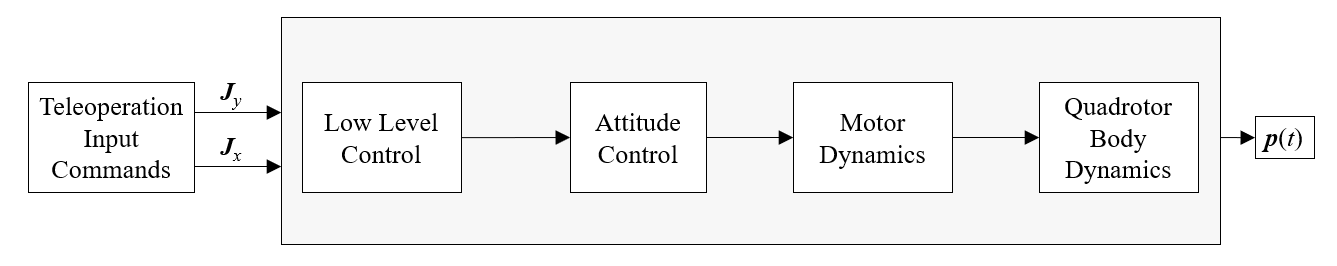
\includegraphics[width=0.48\textwidth]{images/teleopctrl.png}
    \caption{Off-the-Shelf UAV Teleoperation Control Architecture}
    \label{fig:otsctrl}
\end{figure}

The presented structure is a gray box model, where the only information known are the teleoperation inputs, indicated by $\mathbf{J}_x$ and $\mathbf{J}_y$, the output, which is the position of the vehicle, $\mathbf{p}(t)$, over time, and the basic model architecture. The low level controller usually consists of multiple PID loops [CITE], which are already developed and tuned with certain specific control gains, which can be very difficult to identify. The quadrotor body dynamics can be modeled using a $12^{\text{th}}$ order state vector as follows:
%\NB{why q in $\mathbf{p}_q$? In the problem formulation there is not q}
\begin{equation}
    \mathbf{q} = 
    \begin{bmatrix}
    \mathbf{p}^\intercal & \phi & \theta & \psi & v_x & v_y & v_z & \omega_x & \omega_y & \omega_z
    \end{bmatrix}^\intercal \nonumber
\end{equation} 
where $\bm{p}_q=[x \; y \; z]^{\mathsf{T}}$ is the world frame position, $v_{x}$, $v_{y}$ and $v_z$ are the world frame velocities, $\phi$, $\theta$ and $\psi$ are the roll, pitch and yaw Euler angles and $\omega_{x}$, $\omega_{y}$ and $\omega_{z}$ are the body frame angular velocities.

The dynamics of the vehicle are then described as follows:
\begin{equation}
	\begin{aligned}
	%\begin{bmatrix}\dot{x} \\ \dot{y} \\ \dot{z} \end{bmatrix} &= \begin{bmatrix}v_x \\ v_y \\ v_z\end{bmatrix}\\
	\dot{\bm{p}}^{\mathsf{T}} &= \begin{bmatrix}v_x & v_y & v_z\end{bmatrix}\\
	\begin{bmatrix}\dot{v}_x \\ \dot{v}_y \\ \dot{v}_z\end{bmatrix} &= \begin{bmatrix}0 \\ 0 \\ -g \end{bmatrix} + \frac{1}{m} \begin{bmatrix}\cos\phi \cos\psi \sin\theta + \sin\phi \sin\psi \\ \cos\phi \sin\theta \sin\psi - \cos\psi \sin\phi \\ \cos\theta \cos\phi \end{bmatrix} u_1\\
	%\end{align*}
	%\begin{align*}
	\begin{bmatrix}\dot{\phi} \\ \dot{\theta} \\ \dot{\psi}\end{bmatrix} &= \begin{bmatrix}1 & \sin\phi \tan\theta & \cos\phi \tan\theta\\ 0 & \cos\phi & -\sin\phi \\ 0 & \sin\phi \sec\theta & \cos\phi \sec\theta \end{bmatrix} \begin{bmatrix}\omega_{x} \\ \omega_{y} \\ \omega_{z} \end{bmatrix}\\
	\begin{bmatrix}\dot{\omega}_{x} \\ \dot{\omega}_{y} \\ \dot{\omega}_{z}\end{bmatrix} &= \begin{bmatrix}\frac{I_{yy} - I_{zz}}{I_{xx}} \omega_{y}\omega_{z}\\ \frac{I_{zz} - I_{xx}}{I_{yy}} \omega_{x}\omega_{z} \\ \frac{I_{xx} - I_{yy}}{I_{zz}} \omega_{x}\omega_{y} \end{bmatrix} +  \begin{bmatrix}\frac{1}{I_{xx}} & 0 & 0\\ 0 & \frac{1}{I_{yy}} & 0\\ 0 & 0 & \frac{1}{I_{zz}}\end{bmatrix} \begin{bmatrix}u_{2} \\ u_{3} \\ u_{4} \end{bmatrix}
	\end{aligned}
	\label{eq:quadrotor_dynamics} \nonumber
\end{equation} [CITE]

This dynamical model consists of many platform-specific parameters that are also difficult to identify, much like the controller gains discussed above. Moreover, these parameters often vary a lot between UAVs, and that further complicates the identification problem. The model and architecture provided assume that the quadrotor is moving at a constant z level with a zero yaw constraint, and therefore, we are primarily concerned with two of the inputs, $u_2$ and $u_3$. The equations for the control inputs are as follows:
\begin{align} \label{eq:cinputs}
    %u_1 &= m(g + \ddot{z}_{des} + k_{d,z}(\dot{z}_{des}  \dot{z}) + k_{p,z}(z_{des}-z)) \nonumber \\
    u_2 &= k_{p,\phi}(\phi_c-\phi) + k_{d,\phi}(\dot{\phi}_c - \dot{\phi}) \nonumber \\
    \phi_c &= -\frac{1}{g}(\ddot{x}_{des} + k_{d,x}(\dot{x}_{des}-\dot{x}) + k_{p,x}(x_{des}-x)) \nonumber \\
    u_3 &= k_{p,\theta}(\theta_c-\theta) + k_{d,\theta}(\dot{\theta}_c - \dot{\theta}) \nonumber \\
    \theta_c &= -\frac{1}{g}(\ddot{y}_{des} + k_{d,y}(\dot{y}_{des}-\dot{y}) + k_{p,y}(y_{des}-y))
\end{align}
where $\phi_c$ and $\theta_c$ are the desired roll and pitch angles, respectively.

In this work, we are interested in generating control inputs for autonomous flight when the only information available for training comes from human-piloted demonstrations. From the aforementioned demonstrations, we assume that we can obtain position ad the velocity of the system during training as well as the input commands sent to the vehicles from the user teleoperation.
%\NB{this part needs to be rewritten and generalized. We can mention later that in our case we use a MOCAP but here we just need to say that we assume that we can obtain position and velocity of the system during training as well as the commands sent to the vehicles as a result of the user teleop}
%\NB{this is also not true...we are not interested in learning from user. We are levergaing user teleop because it't the only thing we have and we are interested in generating commands for autonomous flight}
Through observation of a single demonstrated trial, we are able to identify important commands sent to the system. An example of this is shown below:

\begin{figure}[ht]
    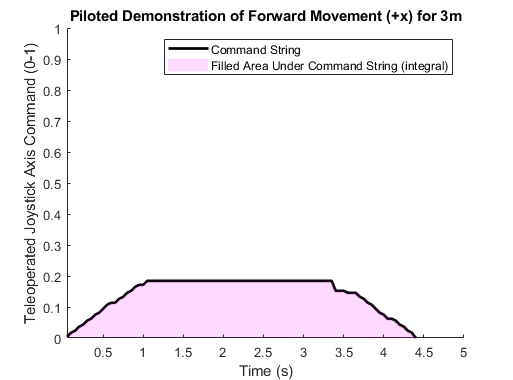
\includegraphics[width=0.48\textwidth]{images/sampleintegral.png}
    \caption{A sample of a single demonstrated flight}
    \label{fig:sampleintegral}
\end{figure}
\NB{we should show this picture in parallel with the speed and position of the vehicle to connect with the integral}
In Fig. \ref{fig:sampleintegral}, we show a sample of a single flight demonstration. The pilot flies the UAV forward over a distance of approximately $3$ meters, with initial and final velocities of $0$. The teleoperation input command string, in this case, corresponds to pitch, where a command of $0$ would imply no pitch adjustment, and $1$ corresponds to the UAV's maximum allowable pitch. The minimum allowable pitch command is $-1$, which would send the UAV in in the negative $y$-direction. 


From \eqref{eq:cinputs}, we can observe that the inputs $u_2$ and $u_3$ for roll and pitch rely on the change in the desired Euler roll and pitch angles, which then rely on the desired $x$ and $y$ positions and velocities. In order to capture that that change in the desired angles, which are set by the human teleoperation, we take the area under the curve of the input commands. The shaded portion of Fig.\ref{fig:sampleintegral} represents this integral. Since these changes in roll and pitch affect the global $x$ and $y$ position of the vehicle, the integral that captures these changes is connected to the distance travelled by the vehicle. This integral is used as a compact measure for our training, and this removes the necessity to train on the entire string of commands, which could be large and more computationally intensive. 

%Along with the string of commands sent, the shaded portion of Fig.\ref{fig:sampleintegral}, represents the integral. i.e. the total area, under the string of commands. Because the pitch is proportional to the linear velocity in the $y$-direction, we know that the command string is proportional to the velocity, and its integral, therefore, is proportional to the distance traveled 
%\NB{here show that because u2 depends on $\phi_c$ and $\phi_c$ depends on x then this integral represents motion but what you really need to stress is that it is a compact measure without having to use the entire string of commands for learning}.

Lastly, the average command sent to the system, as indicated by the dotted line, is of interest. The integral itself, while conveying information about the distance traveled, lacks precision in that the same integral can be achieved with commands strings of different lengths and velocities. Making use of the average teleoperation input command, we are able to identify the correct average autonomous input command and therefore, improve the precision in the process of generating autonomous commands, which must be fixed to a certain length (time) and travel a certain distance. 

%\NB{we need to think how to pose the command better. A reviewer here can still ask why and what so special about the command.}
%\NB{here we need to stress again that these parameters are hard to find online}
%\NB{here we need a model and discussion about the controller}
%The low-level controller, which consists of a series of PID loops [CITE], generate the angle inputs and attitude control that follow the desired trajectory, $\mathbf{p_r}$. The attitude controller and motion dynamics generate the thrust and moment values applied by each rotor. Lastly, the quadrotor body dynamics give the position of the system, which is then fed back into the position controller. This control architecture assumes that the quadrotor is moving at a constant z level with a zero yaw constraint, which is discussed later on in the paper.
%Fig. \ref{fig:ctrl} summarizes the overall control architecture for an autonomous quadrotor.
%\begin{figure}[ht]
%    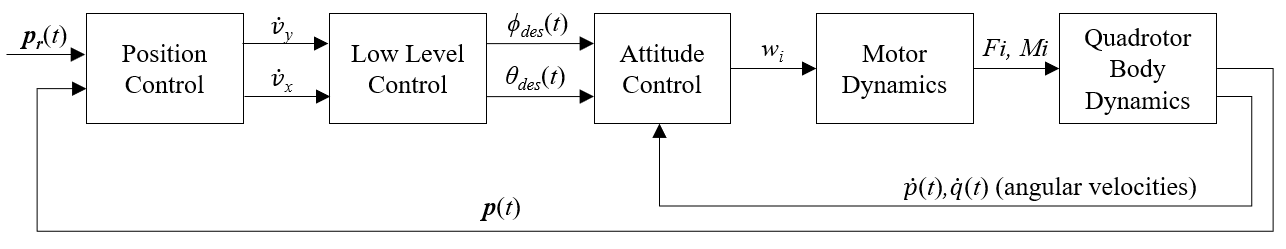
\includegraphics[width=0.48\textwidth]{images/ctrler.png}
%    \caption{UAV Autonomous Control Architecture}
%    \label{fig:ctrl}
%\end{figure}
%Both model parameters and control gains shown above, however, are difficult to identify and can vary a lot from UAV to UAV.
%\NB{here we need to mention that the low level control is typically already developed }
%\NB{this figure should change to include the teleoperation control instead of the position control} \NB{we should include the inner par of the diagram into a gray box and leave outside the joystick commands and the output of the quadrotor.}
%, and the controller architecture shown in Fig.\ref{fig:ctrl} consists of multiple PID loops, and therefore multiple parameters that require platform-specific tuning for autonomous flight and control. It is this requirement that calls for a different method that can be used to enable autonomous flight.

\section{Methodology} \label{sec:approach}

\begin{figure}[ht]
    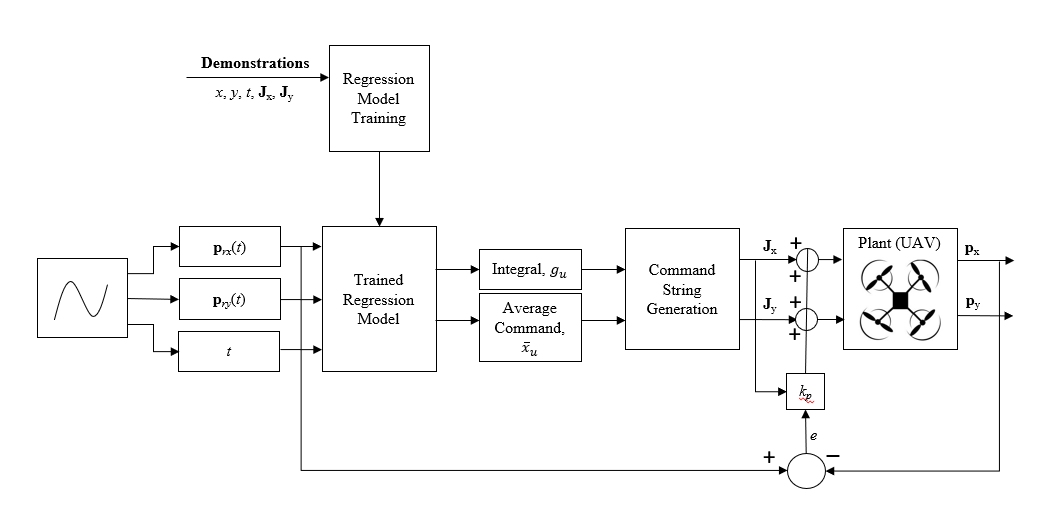
\includegraphics[width=0.48\textwidth]{images/blocks.PNG}
    \caption{Block Diagram of Proposed Approach}
    \label{fig:blockdiagram}
\end{figure}
%\NB{the figure needs to be changed. jx(t) jy(t) should input into the plant and the output is x(t) y(t) and all goes as input to the Training. The figure is still blurry}
%\NB{let's use power point fro the diagrams..it's blurry}


The proposed approach is outlined in Fig.\ref{fig:blockdiagram}. The approach begins with multiple demonstrations that are used to build a regression model that enables identification of the desired integral of the input commands, $g_u$, and desired average teleoperation input command, $\bar{j}_u$, given a user-set target distance, $d_u$, and time, $t_u$. With the integral and average velocity, a new command string consisting of commands for both lateral and longitudinal directions is created using the models within training set. At this stage, we generate the inputs, $\mathbf{J}_x(t)$ and $\mathbf{J}_y(t)$, needed by the system to follow the given trajectory. Because these actions are created in open-loop, accurate trajectory tracking cannot be guaranteed. Tracking error is reduced by closing the loop via a robust control approach to correct and adjust future inputs $\mathbf{J}_x(t+1)$ and $\mathbf{J}_y(t+1)$ to obtain closed loop input commands $\mathbf{J}_{cx}(t+1)$ and $\mathbf{J}_{cy}(t+1)$. First, we will discuss the trajectory decomposition, as our problem ultimately is to accurately track any trajectory.


%\NB{introduce next section... the paper reads like independent sections}
 %\NB{in this section or before we need to stress and clarify that this approach allows us to figure out the actions for the system to follow autonomously any trajectory but we need still to close the loop. Technically is a 2 phase method:1) open loop actions and 2) corrections for closed loop}
\subsection{Trajectory Generation and Decomposition} \label{sec:traj}

In this section, we discuss how a smooth trajectory is generated between waypoints, and how this trajectory is decomposed into $x$ and $y$ components. From the system dynamics, we know that input commands are responsible for specific motions of the system. Roll enables lateral motion while pitch enables longitudinal motion. Therefore, any planar motion assuming constant $z$ and yaw can be represented as a combination of roll and pitch commands, or commands that move the vehicle along the global $x$ and $y$ coordinates. Because the using just roll and pitch commands is possible, we desire to decompose the trajectory into $x$ and $y$ components, as any smooth trajectory can be represented as a combination of these components.

%\NB{this section needs to go before and needs to be explain better}.

In order to generate a trajectory, we first select waypoints through which the UAV should travel. In order to determine the optimal path in our case, we generate a minimum snap trajectory. Minimum snap trajectories are associated with low control effort as they are based on the fourth derivative of position and ensure smoothness \cite{minsnap}. The general equation for a minimum snap trajectory is as follows:
%\NB{why? you need to explain better. Besides, we should use snap not jerk}
\begin{equation} \label{eq:minjerkint}
    \mathbf{p}^*(t) = \argmin_{p(t)}\int_0^T\mathcal{L}(\ddddot{p},\dddot{p},\ddot{p},\dot{p},p,t)dt
\end{equation}

Solving \eqref{eq:minjerkint}, we obtain the form:
\begin{equation}
    \mathbf{p}^*(t) = c_7t^7 + c_6t^6 + c_5t^5 + c_4t^4 + c_3t^3 + c_2t^2 + c_1t + c_0 
\end{equation}
where $c_0,\ldots,c_7$ are constants associated with specific waypoints in the trajectory.
\NB{we need to think if these equations are really necessary here. for now leave them but keep the comment}
Having obtained the smooth trajectory, we then discretize the trajectory into $n$ parts, each of which will have a time-step of $\delta t = \frac{T}{n}$, where $T$ is the total amount of time allotted for the full trajectory. The discretization is done using linear interpolation within the trajectory over the interval $[\mathbf{p}^*(t_s), \mathbf{p}^*(t_{s+1})]$, where $t_s$ is the time at the start of a segment and $t_{s+1}$ is the end of the segment, defined as: $t_{s+1} = t_s + \delta t$. 
%\NB{why so complicated this description...please simplify you are just doing a discretization. Also correct gramamr }.
%\NB{please write the mathematical expression for the x and y component from the trajectory otherwise this section is incomplete}
%\NB{several? they are just 3...please ad the decomposition otherwise this section is useless}
Some examples of decomposed trajectories are shown in Fig.\ref{fig:trajs}. All of the trajectories shown in Fig.\ref{fig:trajs} start at the world frame origin $(0,0)$.

\begin{figure}[h]
	\centering
	\subfigure[\label{fig:t1}]{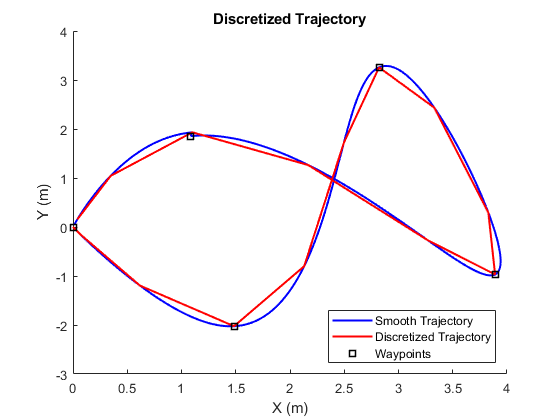
\includegraphics[width=0.3\linewidth]{images/traj1.png}}
	\subfigure[\label{fig:t2}]{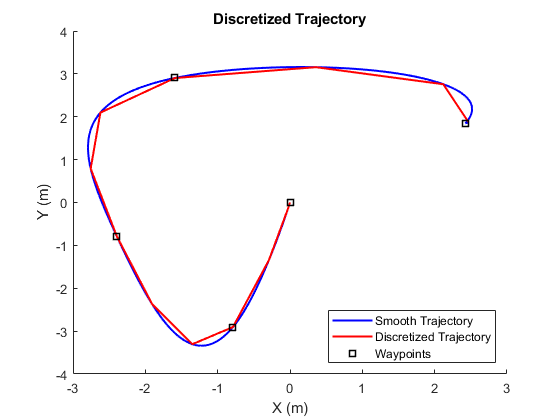
\includegraphics[width=0.3\linewidth]{images/traj2.png}}
    \subfigure[\label{fig:t3}]{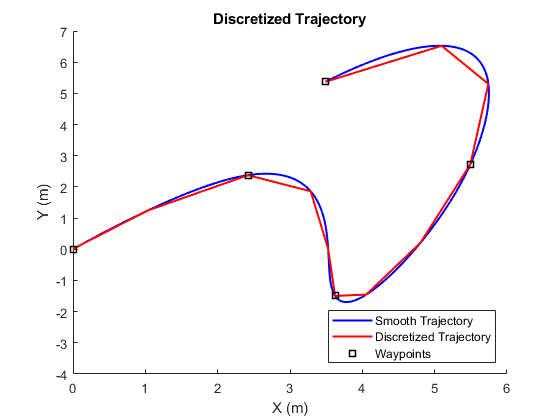
\includegraphics[width=0.3\linewidth]{images/traj3.png}}
	\caption{Discretized Trajectories}
	\label{fig:trajs}
\end{figure}

From the discretized trajectory, we can obtain the $x$ and $y$ components of each leg of the trajectory. Each component is calculated as follows:
\begin{align}
    c_{x}(t_s,t_{s+1}) = \mathbf{p_x}^*(t_{s+1}) - \mathbf{p_x}^*(t_{s}) \nonumber \\
    c_{y}(t_s,t_{s+1}) = \mathbf{p_y}^*(t_{s+1}) - \mathbf{p_y}^*(t_{s})
\end{align}

where $c_{x}(t_s,t_{s+1})$ and $c_{y}(t_s,t_{s+1})$ are the distances between each segment in $x$ and $y$ directions. These values are taken for each of the $n$ trajectory segments with the same time-step, $\delta t$, and are appended to one another to create the desired output for which we will generate input commands. In Fig.~\ref{fig:trajdec}, we show an example of a generated trajectory with its discretization and the $x$ and $y$ components that are stitched together.
\begin{figure}[h]
	\centering
	\subfigure[\label{fig:t2dec}]{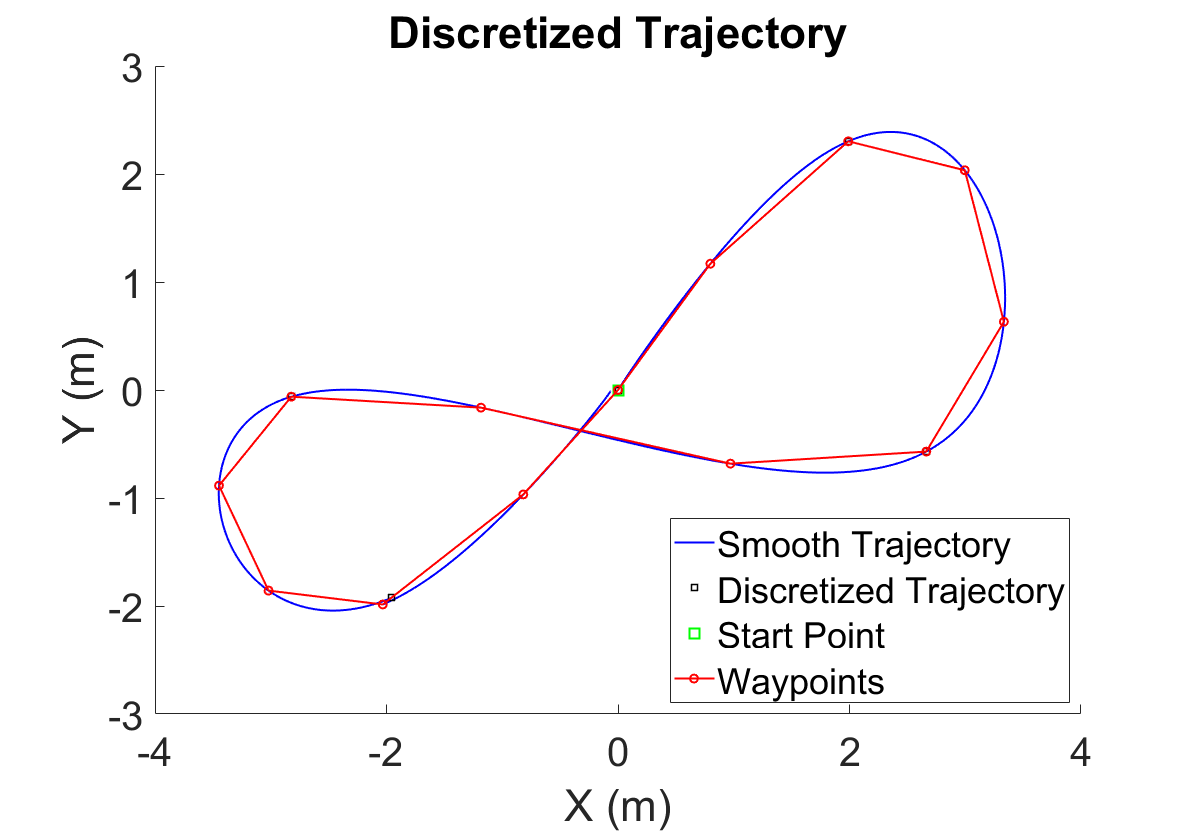
\includegraphics[width=0.48\linewidth]{images/traj2dec.png}}
	\subfigure[\label{fig:tdec}]{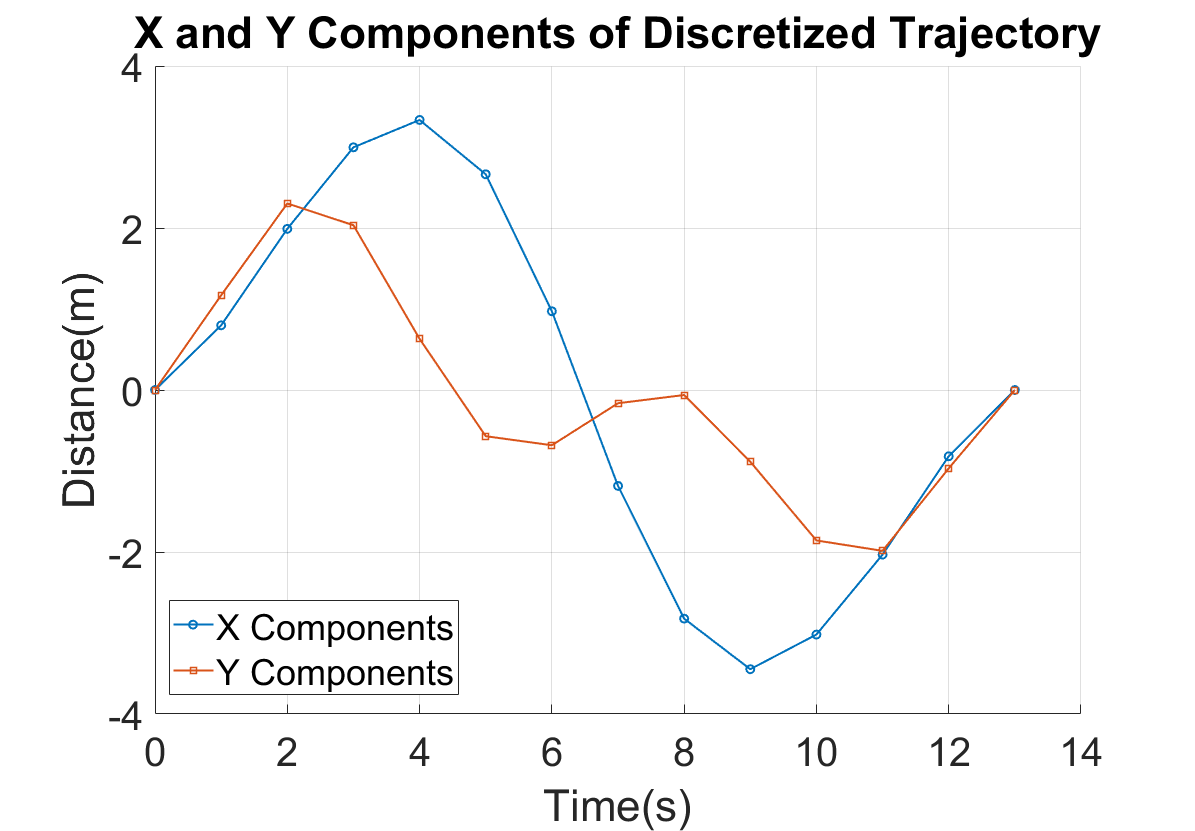
\includegraphics[width=0.48\linewidth]{images/trajdecomp.png}}
	\caption{Example of a Generated Trajectory with its $x,y$ Decomposition}
	\label{fig:trajdec}
\end{figure}

In Fig.~\ref{fig:tdec}, we show the components at each interval. These components, when executed simultaneously, correspond to the trajectory pictured in Fig.~\ref{fig:t2dec}. Having obtained the trajectory $x$ and $y$ components, we will now discuss the training and command generation procedures that we use to build a policy that enables autonomous tracking of the trajectory.


\subsection{Regression Based Training and Evaluation} \label{sec:train}
%\NB{what is this section about? Why do we need this section?}
In order to build the appropriate policy for autonomous command generation, we perform offline training on data collected over $m$ human-piloted trials. As our goal is to track a trajectory, we are interested in training on the distance traveled in the demonstrated trajectory, the time in which the pilot was able to traverse the trajectory, and the sequence of user teleoperation input commands that correspond to the trajectory: $\{d_i,t_i,\mathbf{J_i}\}$, respectively, where $i=1,\ldots,m$ reflects the number of demonstrations. %\NB{what is $i$?}\NB{the reasoning here doesn't make sense. you write that because we need to track a trajectory, we use d and j. This is not intuitive. Why?}.
The outputs of our training phase are \begin{itemize} %should I put Fig 2 and description here instead? It may make more sense, but it's separated from the dynamical model, and that connection is important.
    \item The integral of the string of teleoperation input commands, $g_i = \int_0^{t_i}\mathbf{J}_i$
    \item The average teleoperation input command, $\bar{j}_i \in \mathbf{J}_i$
    \item The position of the system at all times, $\mathbf{p}(t)$
\end{itemize}
%\NB{here it's confusing. Be careful, we are mixing input with outputs.Inout is the distance, time and sequence of commands while the output is the intgeral of the commands, the steady stae teleop, and the state, position, covered by the system}
The average command, in this case, provides information about the pilot's average in-flight velocity, and is obtained by taking the mean of all entries in $\mathbf{J_i}$. The integral, meanwhile, describes the area under the string of commands, as discussed in the previous section.

\subsubsection{Offline Training Data}

Our training data in this work consists of multiple demonstrations of a human-pilot flying forward at varying speeds for varying distances. In Fig.~\ref{fig:train}, we show the raw data received from the demonstrations. In this case, we have training samples where the pilot flies forward and then stops, which is why there are an extended periods where there is no forward motion at the ends of the trajectories in Fig.~\ref{fig:trajs}.

\begin{figure}[ht]
    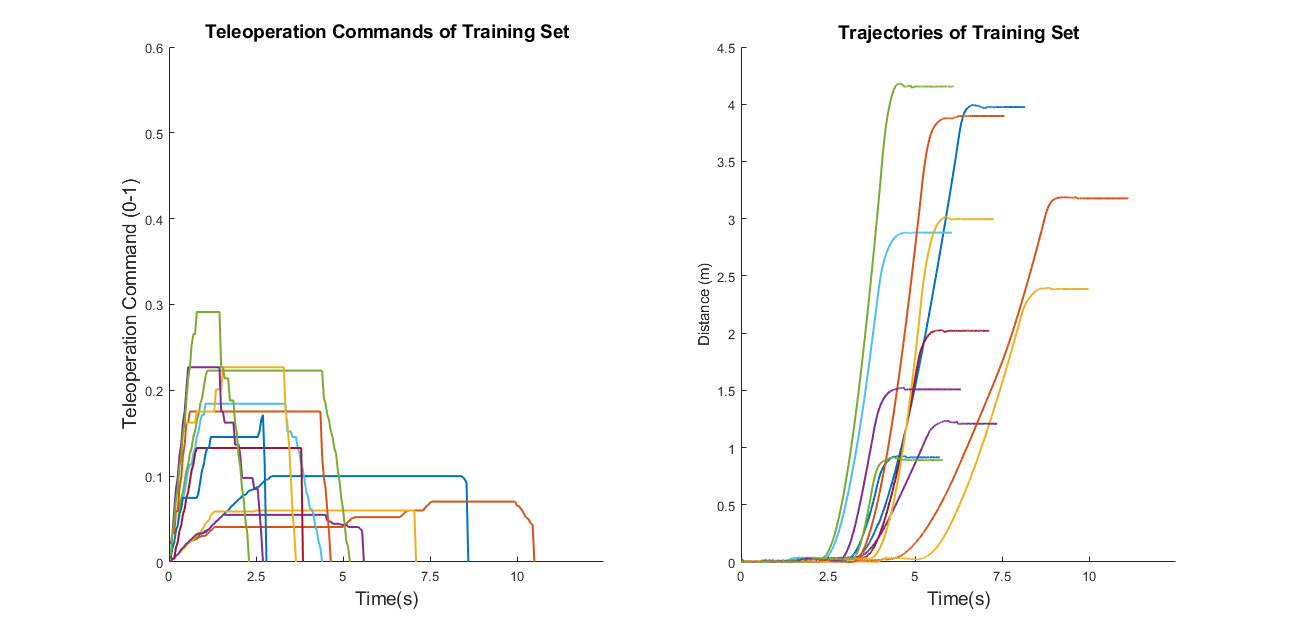
\includegraphics[width=0.48\textwidth]{images/training.png}
    \caption{Training Set, Teleoperation Commands pictured left, Trajectories pictured right}
    \label{fig:train}
\end{figure}

%\NB{rewrite stating that with these data we can train a model for trajectory starting and finishing with 0 speed. If the initial and final velocities are not 0...} 
With this data, we can train a model for trajectories that start and end with $0$ speed. This training would only be effective if trajectories involved stopping intermittently throughout the trajectory. However, we desire a continuous movement between the discretized components of the trajectory. To satisfy this requirement, we segment the training data to include trajectories for demonstrations where the velocity does not start and end at $0$. We are interested in three separate types of segments:
\begin{itemize}
    \item[a.] Trajectory Start, where the segment begins with a velocity of $0$ and ends with a certain nonzero velocity
    \item[b.] Trajectory Intermediate, where the segment begins and end with a certain nonzero velocity
    \item[c.] Trajectory End, where the segment begins with a certain nonzero velocity and ends with a velocity of $0$
\end{itemize}
In order to expand our data for this purpose, we train on portions of the training set pictured in Fig.~\ref{fig:train}, which correspond to each of the three segments we outlined. The segments are formed by cutting the training data and trajectories at the start, the middle, and the end. Shown in Fig.~\ref{fig:trainelab} are four sample from our training set of the velocities and trajectories that correspond to the intermediary segments.
%ewe can extract the aformentioned segments from the training set - cut in a way that way obtain the desired initial and final conditions listed above.
\begin{figure}[h]
	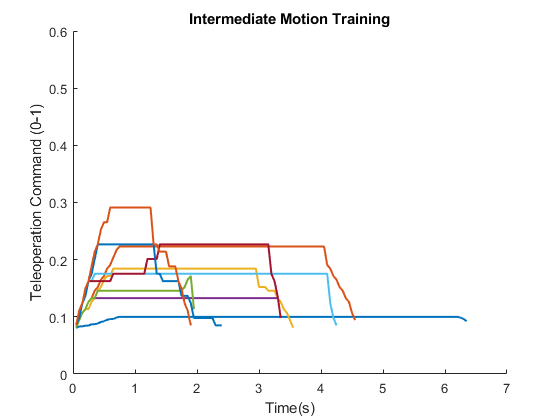
\includegraphics[width=0.48\textwidth]{images/inttrain.png}
	\caption{Training Data with Trajectory Considerations}
	\label{fig:trainelab}
\end{figure}
%change pic to be accurate
Training on not only trajectories that start and end with a velocity of $0$, but also on segments enables more specific command generation based on where the system is in relation to the provided trajectory. For example, if the command for the middle of the trajectory (i.e., between two points that are neither the start nor end of the trajectory) needs to be generated, then the training from the trajectories in Fig.~\ref{fig:trainelab} is used.

%\NB{you are not explaining well how you are doing this}
%\NB{no no no...this is terrible. Delete and rewrite this section from the beginning.}.
%\NB{I'm stopping here for now...the paper needs major changes}

\subsubsection{Thin-Plate Spline Regression Analysis}

The offline training data is applied to a thin-plate spline (TPS) surface regression to describe the relationship between training inputs and integral and average velocity. The general form of a thin-plate spline equation is 
\begin{equation}
    f(x,y) = a_1 + a_xx + a_yy + \sum_{i=1}^mw_iU(||(x_i,y_i)-(x,y)||)
\end{equation}

where $a_1,a_x,\text{and}~a_y$ are scalar coefficients, $w_i$ is a coefficient that corresponds to each specific trial, subject to the following smoothing condition: \begin{equation}
\sum_{i=1}^mw_i=\sum_{i=1}^mw_ix_i=\sum_{i=1}^mw_iy_i=0
\end{equation}
and the function $U$ is of the form
\begin{equation}
  U(r) = r^2\log{r} 
\end{equation}

Given the corresponding $z_i$ for each $(x_i,y_i)$ pair, we solve the following linear system to obtain the coefficients $w_i,\ldots,w_m$ and $a_1,a_x,a_y$,

\begin{equation}
    \begin{bmatrix}
    K&P\\
    P^T& \mathbf{0}
    \end{bmatrix}
    \begin{bmatrix}
    \mathbf{w}\\
    \mathbf{a}
    \end{bmatrix} = 
    \begin{bmatrix}
    \mathbf{z}\\
    \mathbf{o}
    \end{bmatrix}
\end{equation}

where $K_{ij} = U(||(x_i,y_i)-(x_j,y_j)||)$, $P_i* = (1,x_i,y_i)$, $\mathbf{0}  \in \mathbb{R}^{3\times3}$ is a matrix of zeros, $\mathbf{o} \in \mathbb{R}^{3\times1}$ is a column vector of zeros, $\mathbf{w} \in \mathbb{R}^{m\times1}$ and $\mathbf{z} \in \mathbb{R}^{m\times1}$ are formed from $w_i$ and $z_i$, respectively, and $\mathbf{a}$ is the column vector with elements $a_1,a_x,a_y$.

Given the general framework for performing the thin-plate spline, we develop two separate relationships for our specific application. In our work, the first regression is applied to $d$ (distance) and $t$ (time) as inputs to obtain the integral of the commands $g_i = f(d_i,t_i)$ while the second one has the same inputs to obtain the average teleoperation command $\bar{j}_i = h(d_i,t_i)$. With the functions we have obtained, we are able to find an estimated integral and steady-state command, $g_u$ and $\bar{j}_u$, for any given desired distance and time, $d_u$ and $t_u$, respectively,

\begin{equation} \label{eq:integralfit}
g_u = f(d_u,t_u)
\end{equation}
\begin{equation} \label{eq:ssvelfit}
\bar{j}_u = h(d_u,t_u)
\end{equation}

%\NB{PROBLEM: training is performed starting from 0 reaching 0...on a new trajectory online how can you consider different starting velocities? Can we do some considerations on the training? Look among training set, pick all primitives}
In Figs.~\ref{fig:integs} and \ref{fig:joys}, we show the surfaces that represent the two functions $g_i = f(d_i,t_i)$ and $\bar{j}_i = h(d_i,t_i)$, respectively. The points in these figures represent actual training data points, all of which lay on the surface created with the thin-plate spline.

\begin{figure}[ht]
    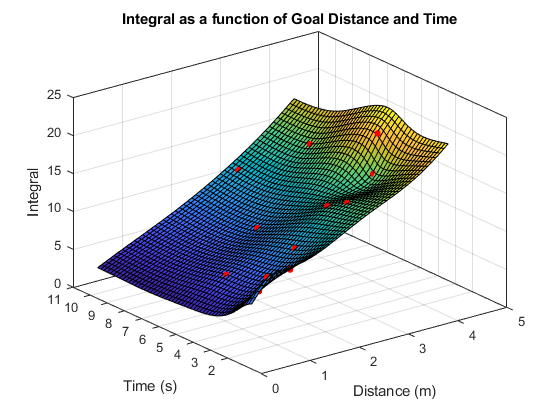
\includegraphics[width=0.48\textwidth]{images/integs.png}
    \caption{Integral vs Distance and Time}
    \label{fig:integs}
\end{figure}
\begin{figure}[ht]
    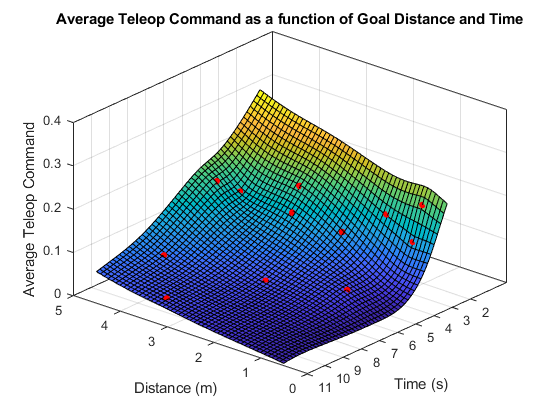
\includegraphics[width=0.48\textwidth]{images/joycmds.png}
    \caption{Average Teleoperation Input Command vs Distance and Time}
    \label{fig:joys}
\end{figure}

While a thin-plate spline is continuous, and a result can be obtained with any combination of distance and time as an input pair, the accuracy of the results of any pair $(d_u,t_u)$ can suffer as the distance between evaluation points and training points increases [CITE]. In order to quantify this, we leverage the standard error of the estimate, which is a statistic used to measure the accuracy of predictions given a certain type of regression \cite{stdereg} with known values:

\begin{equation} \label{eq:stderr}
    \sigma_{est} \approx \frac{s}{\sqrt{m}}
\end{equation}

where $s$ is the sample standard deviation of all of the points in the training set and $m$ is the number of training samples. The standard error, $\sigma_{est}$, is then used to determine the t-statistic for different test values. The t-statistic is defined as the ratio of departure of a test point from a known point to its standard error and is defined as
\begin{equation} \label{eq:tstat}
t_{\hat{\beta}} = \frac{|\hat{\beta}-\bar{\beta}|}{\sigma_{est}}    
\end{equation}
where $\hat{\beta}$ is the test point and $\bar{\beta}$ is the nearest known point. In equation \eqref{eq:tstat}, if $t_{\hat{\beta}} \geq 1$, that means that the test point $\hat{\beta}$ propagates an error higher than the standard error. Therefore, it is desirable to have $t_{\hat{\beta}} < 1$. Using a certain set-point for the t-statistic, the maximum allowable departure from known points is obtained:
\begin{equation}
    \sigma_{est}t_{\hat{\beta}} = |\hat{\beta}-\bar{\beta}|
\end{equation}
This maximum departure, $\sigma_{est}t_{\hat{\beta}}$, is used to set the bounds for each training data point, for example:
\begin{align}
    \hat{\beta}_{\min} = \bar{\beta} - \sigma_{est}t_{\hat{\beta}} \nonumber \\
    \hat{\beta}_{\max} = \bar{\beta} + \sigma_{est}t_{\hat{\beta}}
\end{align}
where $\beta_{\min}$ and $\beta_{\max}$ are the lower and upper bounds for known parameter $\bar{\beta}$.

In our case, there are two inputs we are primarily concerned about for prediction; distance and time. As a result, we perform this calculation twice over, treating each of the two quantities as statistically independent, to obtain maximum departure values for each of the parameters: $\sigma_{d,est}t_{\hat{\beta}}$ and $\sigma_{t,est}t_{\hat{\beta}}$. In \eqref{eq:integralfit} and \eqref{eq:ssvelfit}, the distance and time values are used together as input pairs, so a method to tie the two independent departure values together is desirable. Standard error rectangles \cite{stdellipse}, which create rectangular intervals around each data point, could be used for this purpose, but they are not necessarily accurate for smoothed surfaces, as rectangular regions would have non-differentiable corners, which are incongruous with smoothing conditions met by our TPS regression. An alternative method is to use standard error ellipses, which can be accurately attributed to smooth surfaces as per \cite{stdellipse}. A general equation for a standard error ellipse for our maximum departure is shown below:
\begin{equation}
    \bigg(\frac{x}{\sigma_{d,est}t_{\hat{\beta}}}\bigg)^2 + \bigg(\frac{y}{\sigma_{t,est}t_{\hat{\beta}}}\bigg)^2 = 1
\end{equation}
The ellipses at each point in our training data is calculated using the following parametrized equations:
\begin{align} \label{eq:bounds}
    x_i = d_i + {\sigma_{d,est}t_{\hat{\beta}}}\cos{r} \nonumber \\
    y_i = t_i + {\sigma_{d,est}t_{\hat{\beta}}}\sin{r} 
\end{align}
where $r$ is the parameter in $[0,2\pi]$, and $i = 1,\ldots,m$ and reflects each of the $m$ training samples. Fig.~\ref{fig:preds}, contains a pictorial representation of the standard error ellipses around each point. In Fig.~\ref{fig:predsur}, the surface shown in Fig.~\ref{fig:integs} is modified with a conforming boundary \cite{bounds} created by the ellipses.
\begin{figure}[ht]
	\centering
	\subfigure[Prediction Bounds \label{fig:preds}]{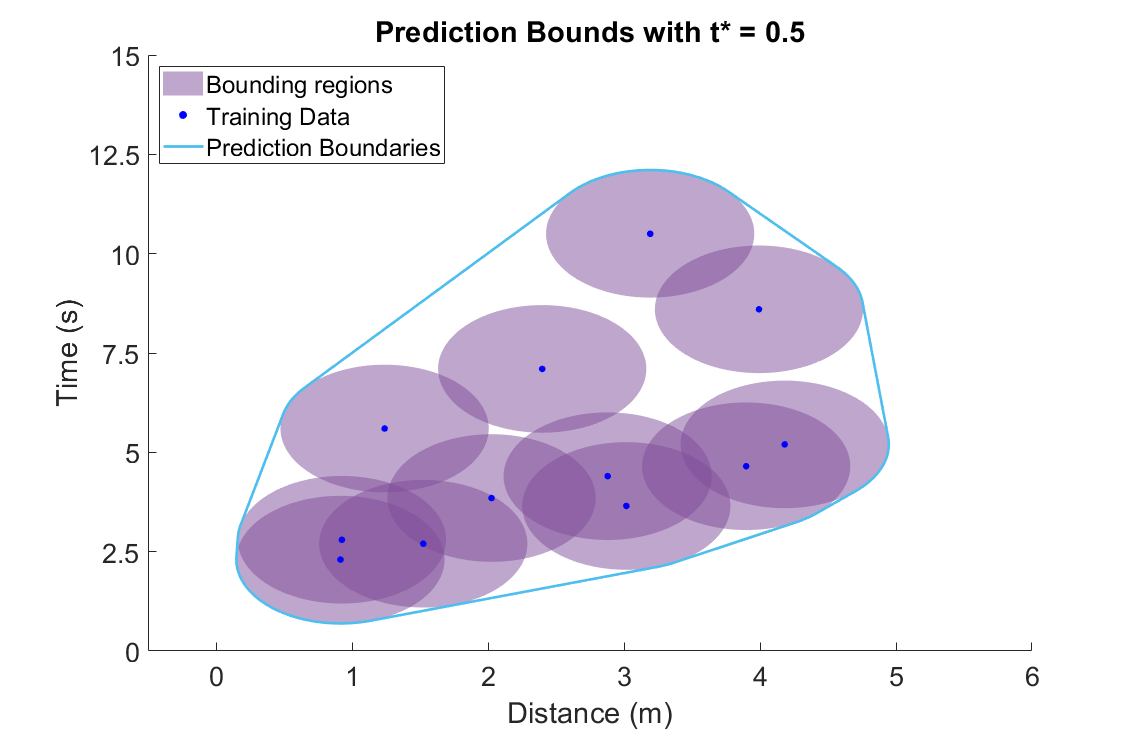
\includegraphics[width=0.48\linewidth]{images/predictionbds.png}}
	\subfigure[Prediction Bounds on Surface \label{fig:predsur}]{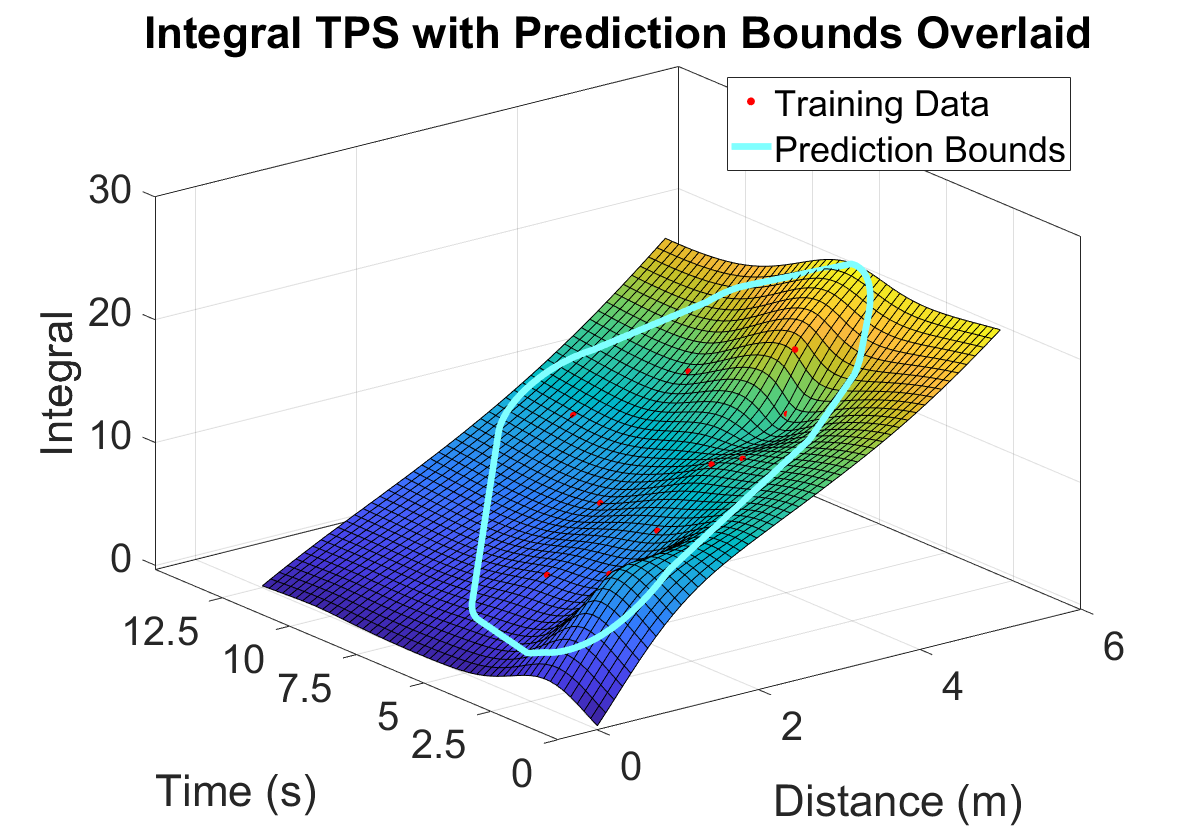
\includegraphics[width=0.48\linewidth]{images/fulpredbds.png}}
	\caption{Prediction Intervals and Bounds}
	\label{fig:bounds}
\end{figure}

Given these prediction bounds, we are able to assess whether or not our trajectory components will have accurate results in the command generation portion of this paper, which follows.

\subsection{Autonomous Input Generation} \label{sec:generate}

In order for the system to autonomously reach a point within trajectory $\mathbf{p_r}(t)$, $g_u$ and $\bar{j}_u$ are obtained using equations \eqref{eq:integralfit} and \eqref{eq:ssvelfit}, and the offline training samples are leveraged to generate a new string of commands. We first check back with our generated trajectory components to ensure that the distances of each segment are within the bounds of our error ellipses, as calculated in \eqref{eq:bounds}, and displayed in Fig.\ref{fig:preds}. If the error regions are violated, we can regenerate a new trajectory or select a different timestep by which to discretize. A string of commands is generated for each component of a trajectory, as described in Section \ref{sec:traj}.

From the training set of $m$ samples, we select the trial that has the closest integral, $g_i$, to the estimated integral $g_u$. This is done by forming an error vector, $\mathbf{e}\in\R^{m}$, where each element is defined by
\begin{equation}
 e_i = \vert g_i-g_u \vert , ~i= \{1,\ldots,m\}
\end{equation}
 The lowest error is then found and is paired with the appropriate pre-trained sample, $\mathbf{J}^*$,
\begin{equation}
\mathbf{J}^* = \mathbf{J}_i \in \mathbf{J}\vert e_i = \min_e(\mathbf{e})
\end{equation}

This optimal pre-trained sample is then adjusted to reflect the user-set time, $t_u$. This is done by performing vector interpolation to re-size $\mathbf{J}^*$, such that important features in the optimal command vector are not lost. These methods are often used for re-sizing complex images, and have shown effectiveness in minimizing feature loss \cite{bicfeatures}. Bicubic interpolation is our chosen method for re-sizing, as it performs better than nearest-neighbor and bilinear interpolation methods, while only marginally increasing computational complexity \cite{biccomp}. The general form of a bicubic interpolation equation is 

\begin{equation} \label{eq:bicinter}
    b(x) = \sum_{i=0}^3a_ij^i
\end{equation}

where $j$ is an entry in vector $\mathbf{J}^*$ and $a$ represents the coefficients of the function at each point. Bicubic interpolation takes the weighted sum of the four nearest neighbors of each entry in the command vector in order to identify a function for the intermediate points between each value in $\mathbf{J}^*$. After resizing, we obtain the time adjusted input vector $\mathbf{J}'$.

The next step is to adjust the input vector such that the system reaches the user-set goal $d_u$. This is done by leveraging the average velocity information, that is, $\bar{j}_u$. Because distance is a function of average velocity and time, the scale time-adjusted vector $\mathbf{J}'$ is scaled such that its mean is equivalent to $\bar{j}_u$. We then obtain

\begin{equation} \label{eq:imgscale}
\mathbf{J}_a = \mathbf{J}'\bigg(\frac{\bar{j}_u}{\bar{j}'}\bigg)
\end{equation}

In Fig.~\ref{fig:gensample}, we show visually the steps of command generation. In Fig.~\ref{fig:ogstring}, we start with the original pre-trained command string that was shown above in Fig.~\ref{fig:sampleintegral}. This flight travelled approximately $4.4$ seconds for $3$ meters. For testing purposes, our use input values are $d_u=3.5$m and $t_u=3.75$s. As indicated, a time adjustment is made first; this is shown in Fig.~\ref{fig:timeadj}. It is important to note that the average command, indicated by the dashed line, is still the same, which is a verification of feature retention using bicubic interpolation from \eqref{eq:bicinter}. If the vector were just stretched without using an interpolation method, we would expect slight variation in the mean, which could damage the integrity of the final step, shown in Fig.~\ref{fig:fullyadj}, which is obtained using \eqref{eq:imgscale}. At this point we have obtained the autonomous command string $\mathbf{J}_a$, which is then sent to the UAV to follow the trajectory $\mathbf{p_r}(t)$.


\begin{figure}[h]
	\centering
	\subfigure[Original String \label{fig:ogstring}]{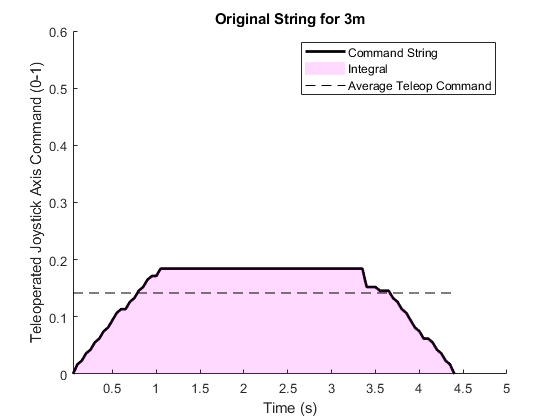
\includegraphics[width=0.3\linewidth]{images/ogstring.png}}
	\subfigure[Time Adjustment \label{fig:timeadj}]{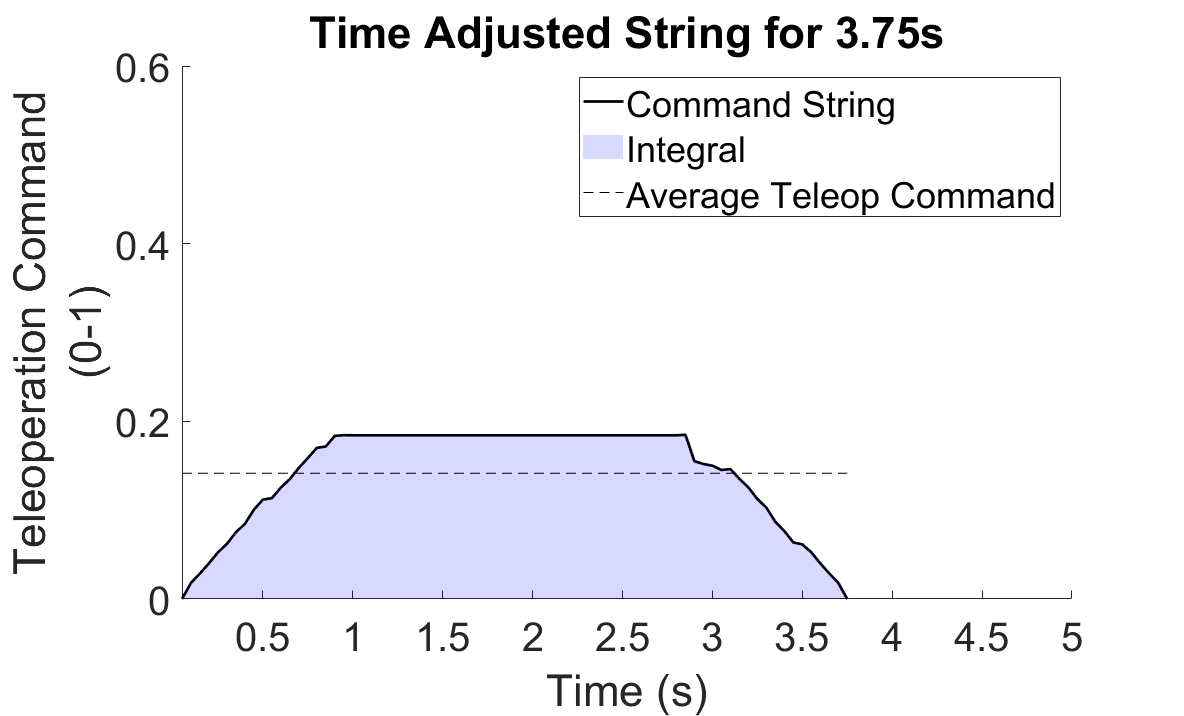
\includegraphics[width=0.3\linewidth]{images/timeadj.png}}
    \subfigure[Final Commands \label{fig:fullyadj}]{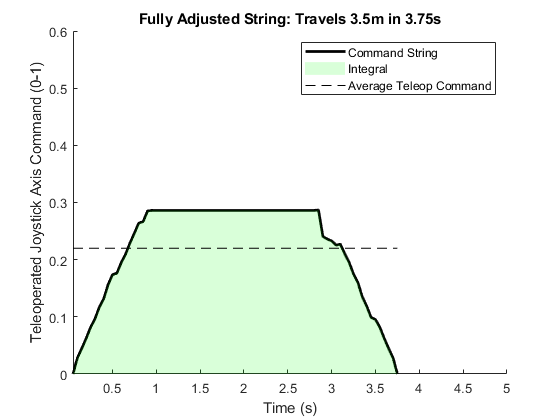
\includegraphics[width=0.3\linewidth]{images/fullyadj.png}}
	\caption{Command Generation Process}
	\label{fig:gensample}
\end{figure}

\subsection{Online Adaptation of Generated Commands} \label{sec:adapt}

The commands generated in the previous section are generated and sent to the UAV in open-loop. In order to close the loop, we propose a method to control for any possible error. While executing generated command string, $\mathbf{x_a}(t)$, we constantly monitor for error between the position of the vehicle, $\mathbf{p}(t)$ and the reference position as per the generated trajectory, $\mathbf{p_r}(t)$:

\begin{equation}
    \xi(t) = \mathbf{p}(t)-\mathbf{p_r}(t)
\end{equation}

The error $\xi(t)$ is attributed to the most recent command $\mathbf{J}_a(t)$, and a proportional controller is used to adjust the following command $\mathbf{J}_a(t+1)$ to obtain the closed-loop command $\mathbf{J}_c(t+1)$ as follows

\begin{equation}
    \mathbf{J}_c(t+1) = \mathbf{J}_a(t+1) + k_p(t)\xi(t)
\end{equation}

The proportional gain, $k_p(t)$, is automatically tuned based using a gradient descent method where the proportional gain is adjusted until the position error, $\xi(t)$ converges to $0$. The initial value of our gain, $k_p$ is set to $0$, which indicates that we assume 

\begin{equation}
    k_p(t+1) = k_p(t) + \frac{\xi(t)}{\mathbf{p_r}(t)}
\end{equation}

The quantity $\frac{\xi(t)}{\mathbf{p_r}(t)}$ relates the current error to the desired position within the trajectory. 


%where $t_u$ refers to the user-set time, and adjusts the update of $k_p$ such that the rate of increase is controlled for iteration time. If the rate of increase is not controlled in this manner, it would suggest that the controller is controlling for error over the entire remaining string of commands, rather than the first subsequent command. Each subsequent command is adjusted because our positional liveness constraint is defined as maintaining a certain distance between actual and reference positions at all times, from \eqref{eq:positlive}. If the constraint was for the UAV to reach the goal at a certain time immaterial of the path/trajectory, adjusting the entire remaining portion of the command string would be ideal.


\section{Experiments} \label{sec:exper}

The proposed approach was validated experimentally using an Parrot Bebop 2 Drone quadrotor UAV, which arrives tuned and stable for teleoperation off-the-shelf. Since experiments were conducted indoors, a Vicon motion capture system was used to obtain the position and velocity of the vehicle. The teleoperation was performed using a node written in the ROS environment.

First, we will discuss how training samples were generated. A human teleoperated the system for 12 samples of motion that only consisted of pitch commands. These training trajectories had different distances and took different amounts of time. We were also able to use this same training set to generate roll commands. The regression and error analysis was done in MATLAB to obtain the surfaces pictured in Section \ref{sec:train} Figs.~\ref{fig:integs} and \ref{fig:joys}.



\section{Conclusions} \label{sec:conc}
In this work, we have presented an approach that enable autonomous flight on off-the-shelf quadrotors that are primarily tuned for teleoperation. Our approach shows that we can use a small training set along with a regression analysis to generate commands for any trajectory, with minimal knowledge of the control architecture and specific dynamical parameters. 



\section{Acknowledgement}


\addtolength{\textheight}{-12cm}   % This command serves to balance the column lengths
                                  % on the last page of the document manually. It shortens
                                  % the textheight of the last page by a suitable amount.
                                  % This command does not take effect until the next page
                                  % so it should come on the page before the last. Make
                                  % sure that you do not shorten the textheight too much.

%%%%%%%%%%%%%%%%%%%%%%%%%%%%%%%%%%%%%%%%%%%%%%%%%%%%%%%%%%%%%%%%%%%%%%%%%%%%%%%%

%References are important to the reader; therefore, each citation must be complete and correct. If at all possible, references should be commonly available publications.




\bibliographystyle{IEEEtran}
\bibliography{bib}




\end{document}
